\documentclass[border=10pt]{standalone}

\usepackage{tikz}
\usepackage{tikzsymbols}
\usetikzlibrary{calc,patterns,shapes.geometric}

\def\centerarc[#1](#2)(#3:#4:#5){\draw[#1] ($(#2)+({#5*cos(#3)},{#5*sin(#3)})$) arc (#3:#4:#5);}

\begin{document}
	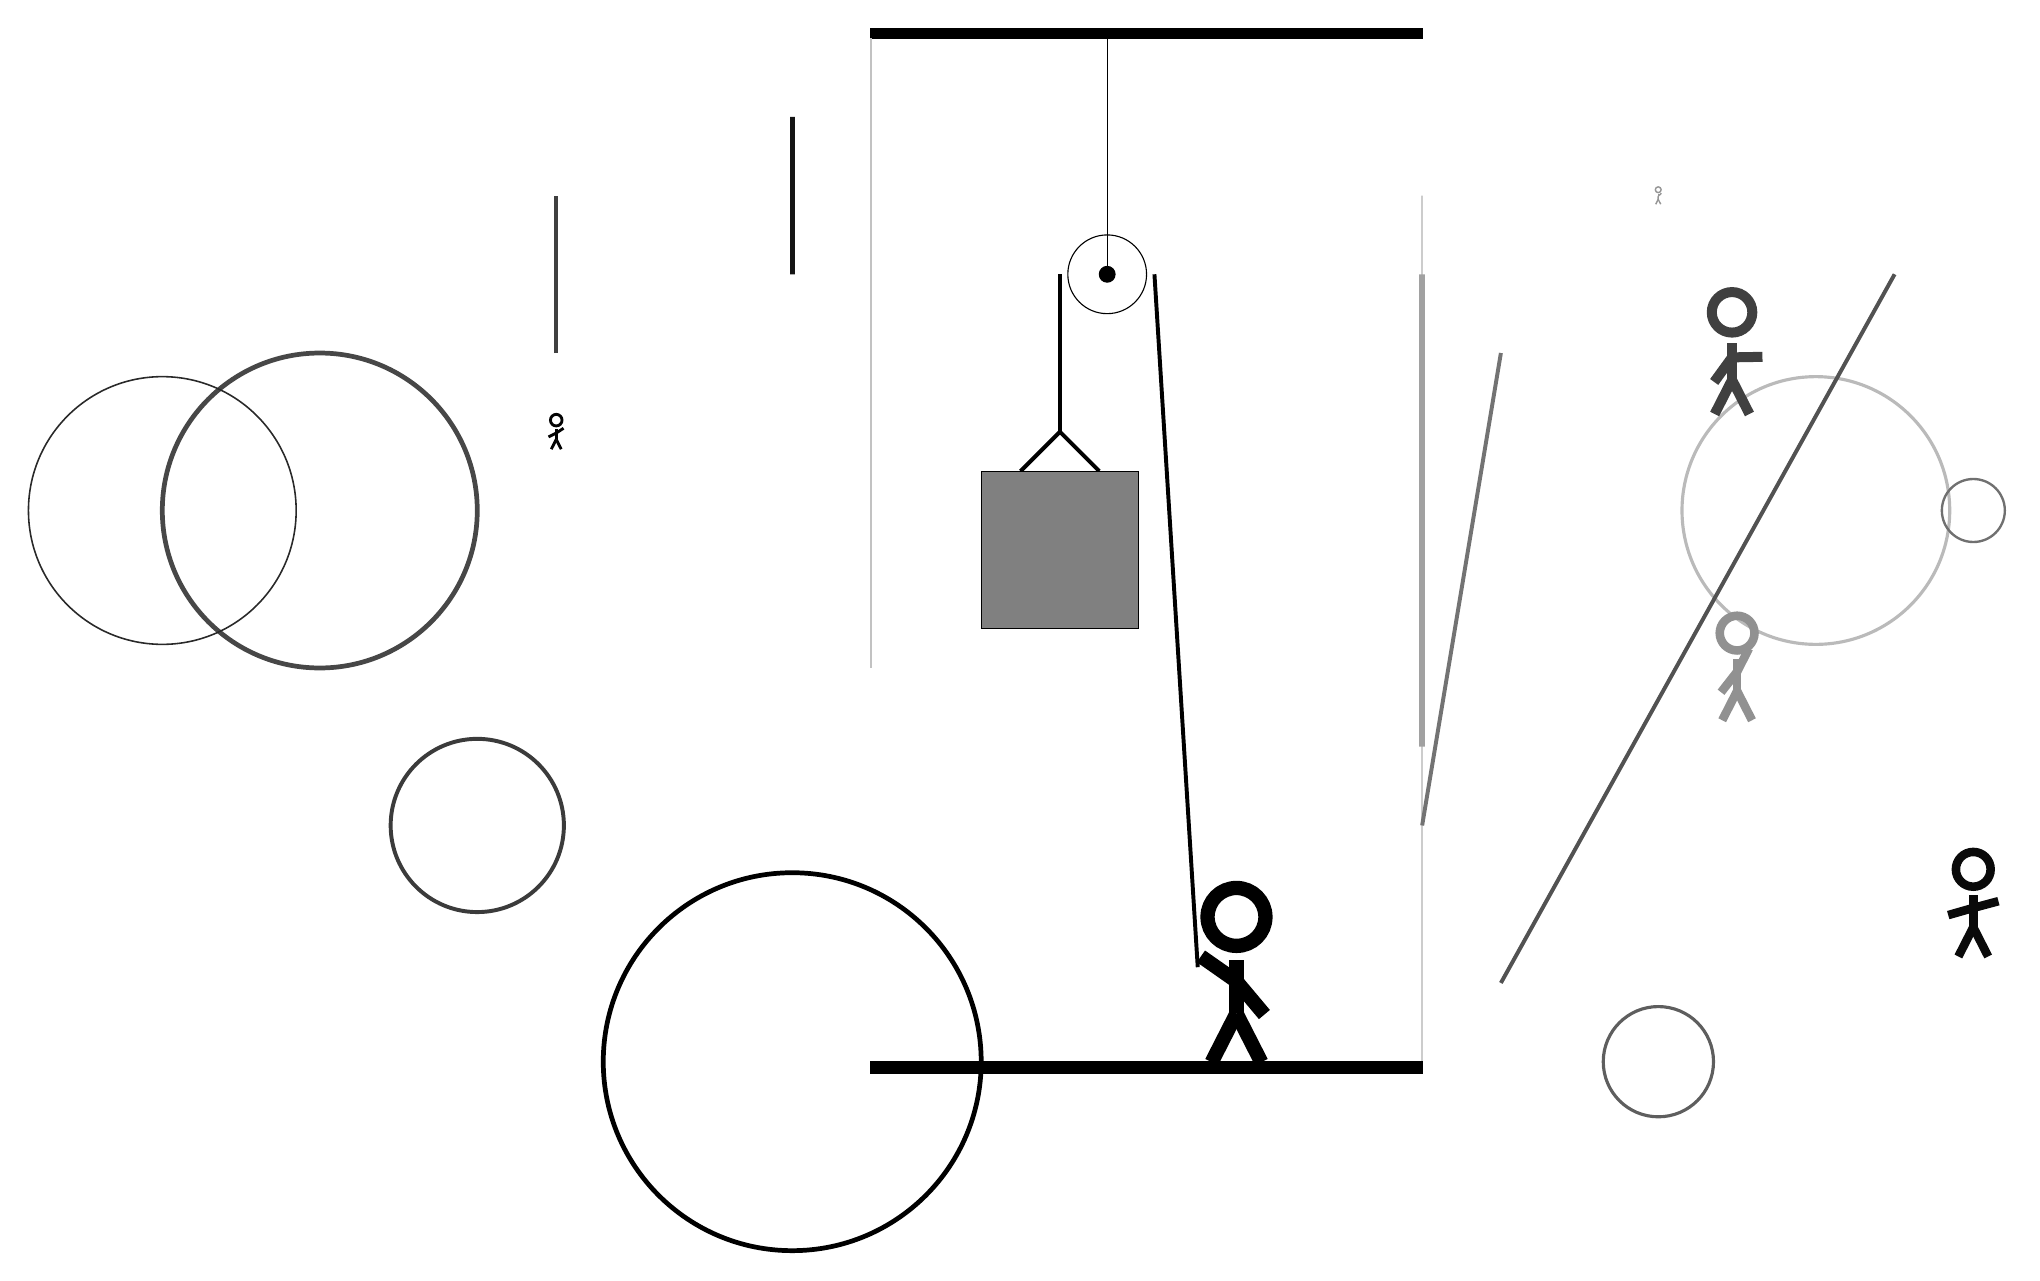
\begin{tikzpicture}
		%%%%% START %%%%%
		
		\draw[fill=black] (-2, 10) rectangle (5, 10.125);
		
		\draw [line width=0.4mm, color=black!27](10, 4) circle (1.7);
		
		\draw[line width=0.3mm, color=black!20] (5, 8) rectangle (5, -3);
		\draw [line width=0.3mm, color=black!56](12, 4) circle (0.4);
		\draw [line width=0.6mm, color=black!100](-3, -3) circle (2.4);
		
		\draw [line width=0.5mm, color=black!77](-7, 0) circle (1.1);
		\draw[line width=0.5mm, color=black!55](5, 0) -- (6, 6);
		
		\draw [line width=0.6mm, color=black!72](-9, 4) circle (2.0);
		\node[line width=0.6mm, color=black!99] at (-6, 5) {\Strichmaxerl[2][27][33]};
		\node[line width=0.4mm, color=black!43] at (9, 2) {\Strichmaxerl[6][52][63]};
		\draw [line width=0.2mm, color=black!84](-11, 4) circle (1.7);
		\draw[line width=0.6mm, color=black!92] (-3, 9) rectangle (-3, 7);
		\draw[line width=0.5mm, color=black!75](-6, 6) -- (-6, 8);
		\draw[line width=0.7mm, color=black!37] (5, 1) rectangle (5, 7);
		
		\draw[line width=0.3mm, color=black!24] (-2, 10) rectangle (-2, 2);
		\node[line width=0.2mm, color=black!41] at (8, 8) {\Strichmaxerl[1][87][43]};
		\draw[line width=0.5mm, color=black!68](6, -2) -- (11, 7);
		
		\draw [line width=0.4mm, color=black!63](8, -3) circle (0.7);
		\node[line width=0.5mm, color=black!75] at (9, 6) {\Strichmaxerl[7][54][1]};
		\node[line width=0.7mm, color=black!96] at (12, -1) {\Strichmaxerl[6][16][15]};
		
		\draw (1, 7) circle (0.5);
		\draw[fill=black] (1, 7) circle (0.1);
		\draw (1, 10) -- (1, 7);
		
		\draw[line width=0.5mm] (-0.1, 4.5) -- (0.4, 5.0) -- (0.9, 4.5);
		\draw[fill=black!50] (-0.6, 4.5) rectangle (1.4, 2.5);
		
		\draw[line width=0.5mm] (0.4, 7) -- (0.4, 5.0);
		\centerarc[line width=0.5mm](1, 7)(0:180:0.6);
		\draw[line width=0.5mm](1.6, 7) -- (2.15, -1.8);
		
		\node at (2.6, -1.9) {\Strichmaxerl[10][-35][-50]};
		
		\draw[fill=black] (-2, -3) rectangle (5, -3.15);
		
		%%%%% END %%%%%
	\end{tikzpicture}
\end{document}